
\documentclass{article}
\usepackage[frenchb]{babel}
\usepackage[T1]{fontenc}
\usepackage[utf8]{inputenc}
\usepackage{soul}
\usepackage{listings}
\usepackage{lmodern}
\usepackage[colorlinks=true, linkcolor=blue]{hyperref}
\usepackage[a4paper, width=150mm, top=25mm, bottom=25mm]{geometry}
\usepackage{parskip}
\usepackage{enumitem}
\usepackage{titlesec}

\usepackage{listings}
\usepackage{xcolor}

\lstset{
	language=Java,
	breaklines=true,
	breakatwhitespace=true,
	basicstyle=\small\ttfamily,
	numbers=left,
	numberstyle=\tiny,
	frame=single,
	showstringspaces=false,
	tabsize=2,
	keywordstyle=\color{red},
}

\usepackage[final]{pdfpages}
\setlist[itemize]{label=\textbullet}
\usepackage{fancyhdr}
\pagestyle{fancy}
\fancyhead{}
\fancyhead[C]{\leftmark}
\renewcommand{\headrulewidth}{0.4pt}
\renewcommand{\footrulewidth}{0.4pt}

\begin{document}
	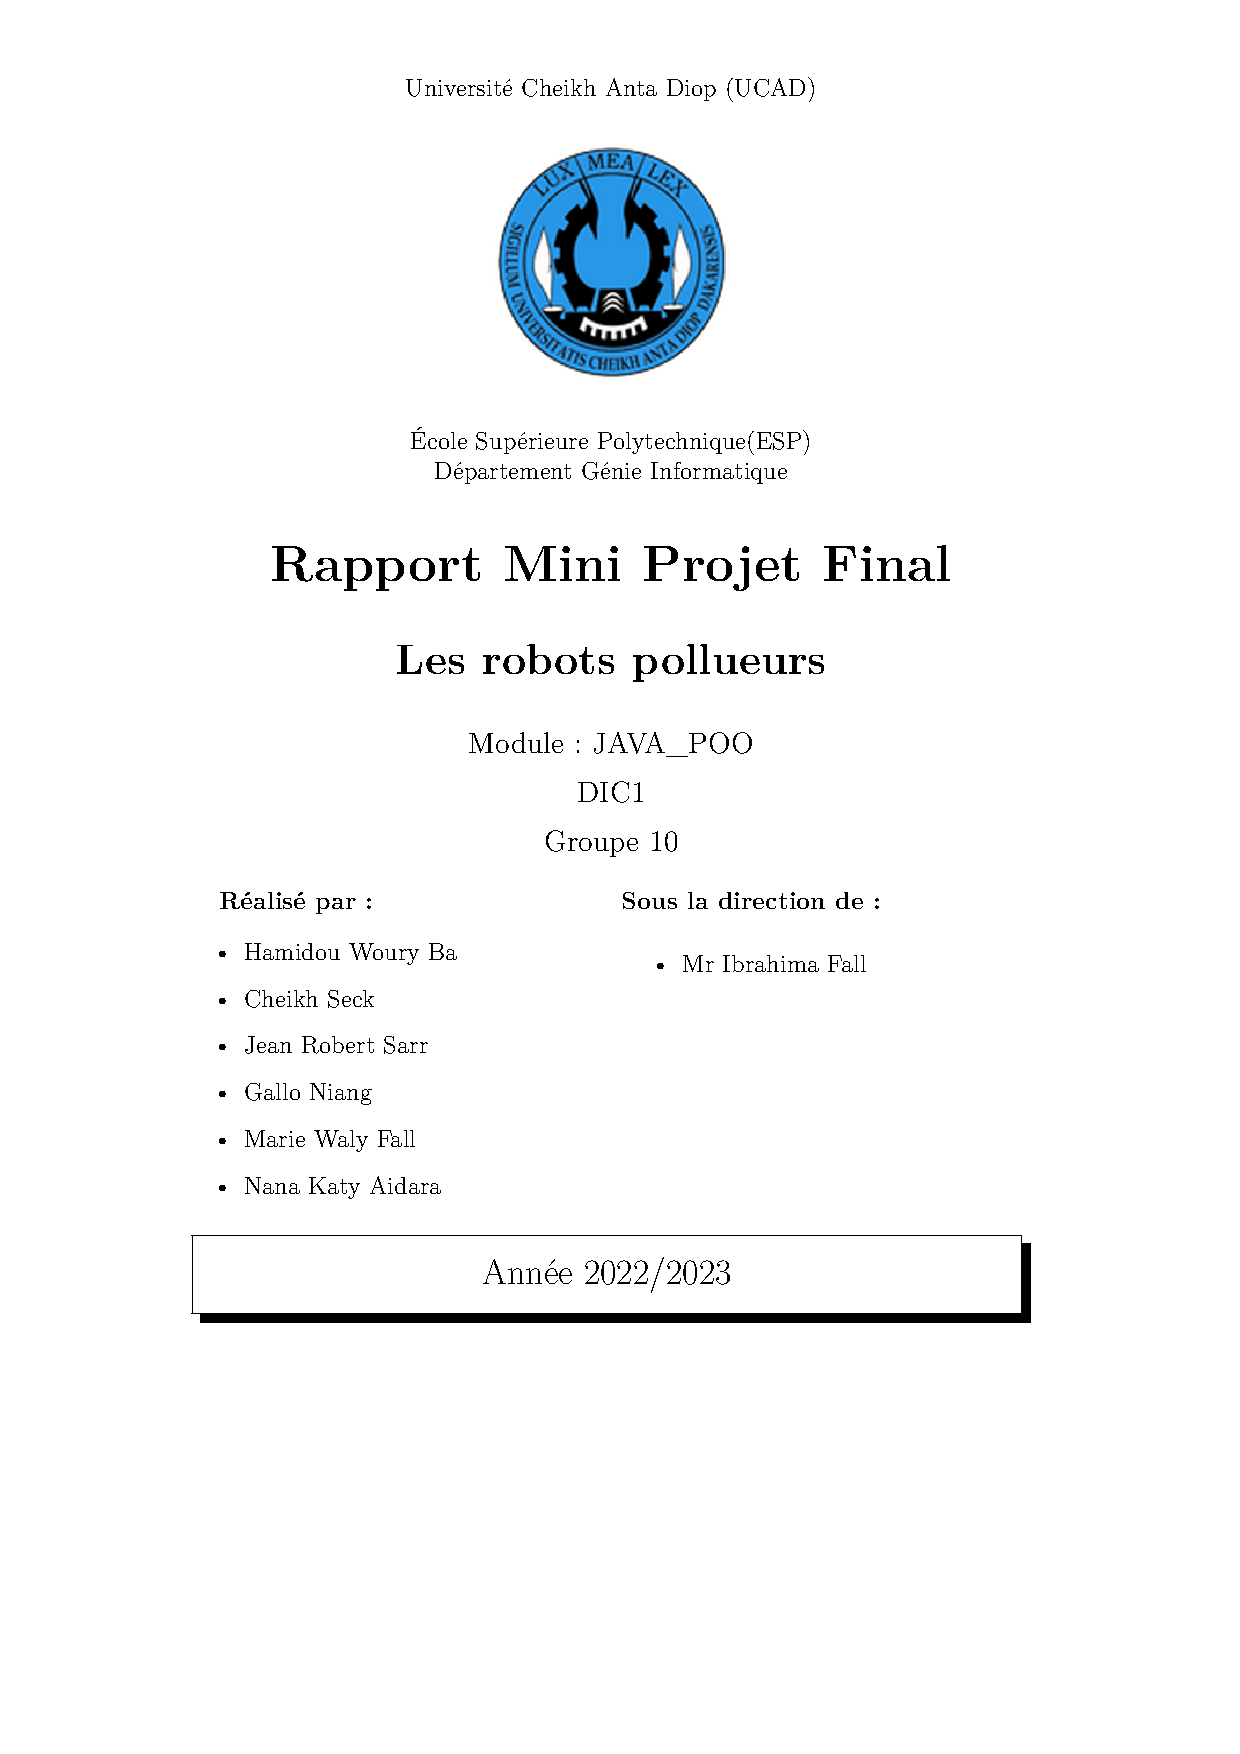
\includepdf[pages=1]{pagedegarde.pdf} 
	\textcolor{red}{\section*{Les classes et méthodes}}
	Nous avons 8 classes à savoir :
	\begin{enumerate}
		\item La classe \textbf{Monde} qui est constituée de 6 méthodes:
		\begin{enumerate}
			\item La méthode \textbf{toString} : cette méthode retourne une chaîne de caractères décrivant le monde.
			\item La méthode \textbf{estValide} : cette méthode permet de vérifier que la case demandée appartient à la matrice.
			\item La méthode \textbf{metPapierGras} : cette méthode met un papier gras dans la case (i; j).
			\item La méthode \textbf{prendPapierGras} : cette méthode enlève le papier gras de la case (i; j).
			\item La méthode \textbf{estSale} : cette méthode teste si la case (i, j) a un papier gras.
			\item La méthode \textbf{nbPapiersGras} : cette méthode rend le nombre de papier gras dans le monde.
		\end{enumerate}
		\item La classe \textbf{Robot} qui est une classe abstraite, elle est constituée de 3 méthodes :
		\begin{enumerate}
			\item La méthode \textbf{estValide} : cette méthode permet de vérifier que la case demandée appartient à la matrice.
			\item La méthode \textbf{vaEn} : cette méthode se déplace en (i, j).
			\item La méthode \textbf{parcourir} : cette méthode permet aux robots de parcourir le monde. 
			Comme chaque robot a sa manière de parcourir le monde , on devra donc l'implémenter selon cette condition dans les sous-classes.
		\end{enumerate}
		\item La classe \textbf{PollueurToutDroit} qui hérite de \textbf{Robotpollueur}, donc elle hérite des méthodes et attributs de la classe \textbf{RobotPollueur}. Puisqu' elle hérite d'une classe abstraite, nous avons redéfinit la méthode abstraite \textbf{parcourir}.
		\item La classe \textbf{Robotpollueur} en plus d'être une classe abstraite , elle hérite de la classe \textbf{Robot}, donc elle hérite de tous les attributs et de toutes les méthodes de sa classe mère.
		Elle possède également une autre méthode :
		\begin{enumerate}
			\item La méthode \textbf{polluer} :cette méthode met un	papier	gras là	où ce robot se trouve dans le monde.
		\end{enumerate}
		\item La classe \textbf{PollueurSauteur} qui hérite de \textbf{Robotpollueur}, donc elle hérite des méthodes et attributs de la classe \textbf{RobotPollueur}. Puisque \textbf{PollueurSauteur} hérite d'une classe abstraite, nous avons redéfinit la méthode abstraite \textbf{parcourir}.
		\item La classe \textbf{RobotNettoyeur} qui hérite de \textbf{Robot}, donc elle hérite des méthodes et attributs de la classe \textbf{Robot}. Puisque \textbf{PollueurNettoyeur} hérite d'une classe abstraite, nous avons redéfinit la méthode abstraite \textbf{parcourir}.
		Cette classe possède également une autre méthode :
		\begin{enumerate}
			\item La méthode \textbf{nettoyer} : enlève	le	papier gras de	la	case où se trouve ce robot.
		\end{enumerate}
		\item La classe \textbf{NettoyeurDistrait} qui hérite de \textbf{Robot}, donc elle hérite des méthodes et attributs de la classe \textbf{Robot}. Puisque \textbf{PollueurDistrait} hérite d'une classe abstraite, nous avons redéfinit la méthode abstraite \textbf{parcourir}.
		\item La classe \textbf{TestRobots} : cette classe contient	un	programme	de	test	des	classes	précédentes.
	\end{enumerate}
\textbf{Remarque :} Chaque classe est constituée d'un ou de deux constructeurs sauf la classe TestRobots
	\newpage
	\textcolor{red}{\section*{Code des classes}}
	\textcolor{red}{\subsection*{Code de la classe Monde.java}}
	\lstinputlisting[inputencoding=utf8]{../Mondepackage/Monde.java}
	\textcolor{red}{\subsection*{Codes de la classe Robot.java}}
	\lstinputlisting[inputencoding=utf8]{../Robotpackage/Robot.java}
	\textcolor{red}{\subsection*{Codes de la classe RobotPollueur}}
	\lstinputlisting[inputencoding=utf8]{../RobotPollueurpackage/RobotPollueur.java}
	\textcolor{red}{\subsection*{Code de la classe PollueurSauteur.java}}
	\lstinputlisting[inputencoding=utf8]{../PollueurSauteurpackage/PollueurSauteur.java}
	\textcolor{red}{\subsection*{Codes de la classe PollueurToutDroit.java}}
	\lstinputlisting[inputencoding=utf8]{../PollueurToutDroitpackage/PollueurToutDroit.java}
	\textcolor{red}{\subsection*{Codes de la classe RobotNettoyeur.java}}
	\lstinputlisting[inputencoding=utf8]{../RobotNettoyeurpackage/RobotNettoyeur.java}
	\textcolor{red}{\subsection*{Codes de la classe NettoyeurDistrait.java}}
	\lstinputlisting[inputencoding=utf8]{../NettoyeurDistraitpackage/NettoyeurDistrait.java}
	\textcolor{red}{\subsection*{Codes de la classe TestRobots.java}}
	\lstinputlisting[inputencoding=utf8]{../TestRobots.java}

\textcolor{red}{\section*{Tests et Captures}}
\textcolor{red}{\textbf{\Large{Exercice 1 :}}}\\

Il s'agissait ici de créer la classe Monde avec les différentes méthodes citées ci-dessus :
\begin{lstlisting}
// Creation du monde
Monde monde = new Monde();
System.out.println("\n");
System.out.println("+----------------+");
System.out.println("| CLASSE : Monde |");
System.out.println("+----------------+\n");

// Test de la classe Monde
System.out.println("Testons la methode metPapierGras aux coordonnees (1,1) et (1,2)");
monde.metPapierGras(1, 1);
monde.metPapierGras(1, 2);
System.out.println(monde.toString());
System.out.print("Testons la methode estSale aux coordonnees (1,1) : ");
System.out.println(monde.estSale(1, 1));
System.out.println("Le nombre de papiers gras dans le monde : " + monde.nbPapiersGras());
}\end{lstlisting}
Dans ce code nous avons créé un objet monde en utilisant le constructeur sans paramètre.\\
Par la suite, nous appelons la méthode \textbf{metPapierGras} sur l'objet créé pour qu'il puisse mettre des papiers gras sur les positions données en paramètres.\\
On affiche le monde en appelant la méthode \textbf{toString}.\\
Après nous appelons la méthode \textbf{estSale} pour vérifier si la case (1,1) est sale. \\
Enfin, nous appelons la méthode \textbf{nbPapiersGras} pour compter le nombre de papiers gras dans le monde.\\

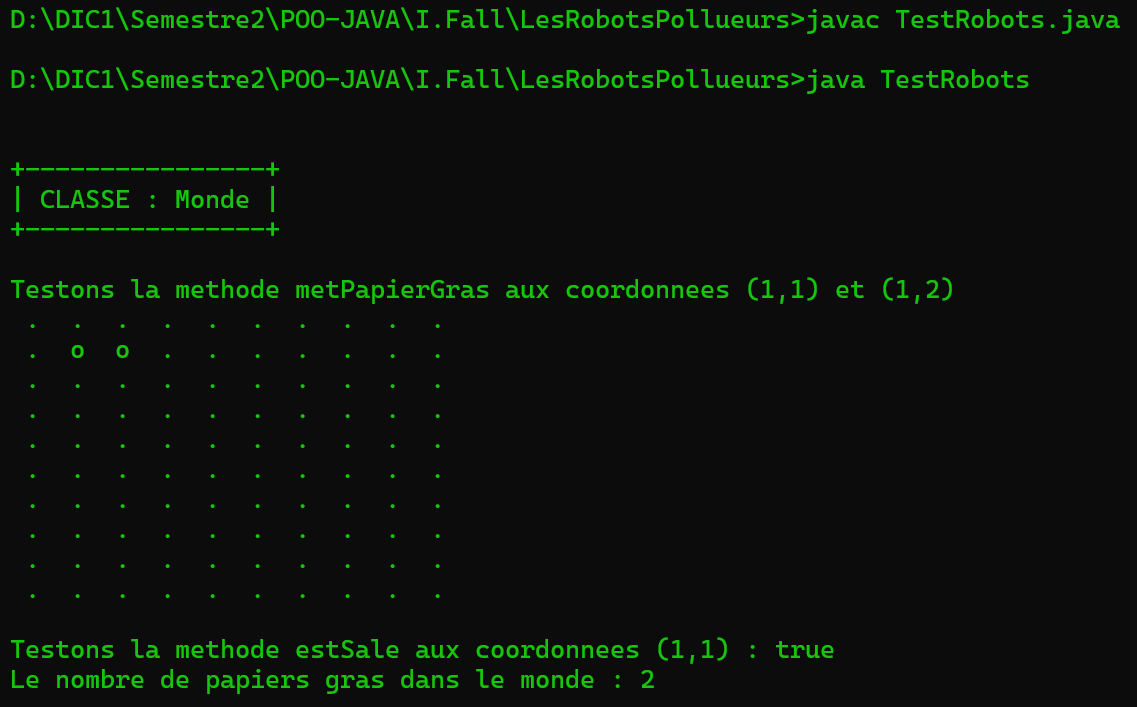
\includegraphics[scale=0.5]{../images/exo1.png}\\

On voit bien l'appel de la méthode \textbf{metPapierGras} (2 fois) a permis de mettre des papiers gras dans le monde dans les différentes positions données en paramètre.\\
En bas on voit \textbf{true}, c'est parceque l'appel de la méthode \textbf{estSale} avec comme paramètre (1,1) montre qu'au niveau de cette case il y a présence de papier gras.\\
On voit bien que le nombre de papiers gras dans le monde est 2.

\begin{lstlisting}
System.out.println("Testons la methode prendPapierGras aux coordonnees (1,1)");
monde.prendPapierGras(1, 1);
System.out.println(monde.toString());
System.out.println("Le nombre de papiers gras dans le monde : " + monde.nbPapiersGras());
System.out.println("\n\n\n");
}\end{lstlisting}

Maintenant dans le code ci-dessus, on va essayer de tester la méthode \textbf{prendPapierGras}.
Puis on affiche le monde et compte le nombre de papiers gras.

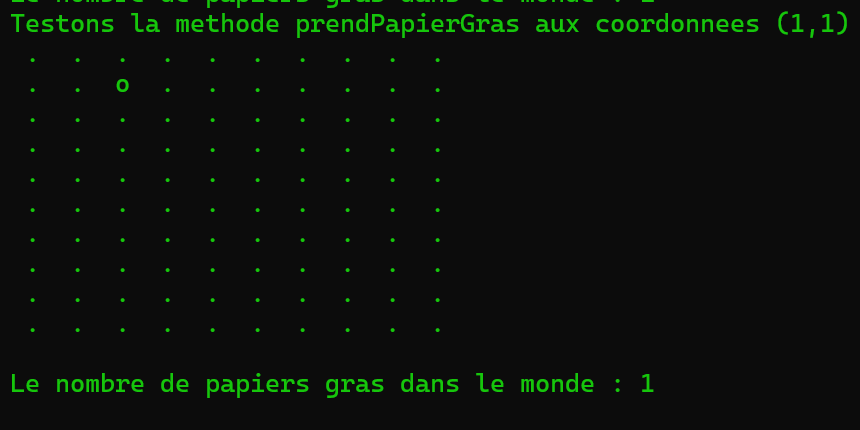
\includegraphics[scale=0.5]{../images/exo1.1.png}\\

On voit bien que la méthode \textbf{prendPapierGras} enlève le papier gras de la position (1,1) et le nombre de papier gras revient 1.\\

\textcolor{red}{\textbf{\Large{Exercice 2 :}}}\\
Il s'agissait ici de créer la classe \textbf{Robot} (classe abstraite) avec les différentes méthodes citées ci-dessus.\\
Puisque la classe \textbf{Robot} est abstraite, on ne peut pas l'instancier.\\

\textcolor{red}{\textbf{\Large{Exercice 3 :}}}\\
Il s'agissait ici de créer la classe \textbf{RobotPollueur} (classe abstraite) avec les différentes méthodes citées ci-dessus.\\
Cette classe également est abstraite, on ne peut pas l'instancier.\\

\textcolor{red}{\textbf{\Large{Exercice 4 :}}}\\
Il s'agissait ici de créer la classe \textbf{PollueurToutDroit} avec les différentes méthodes citées ci-dessus.\\
\begin{lstlisting}
	//Test de la classe PollueurToutDroit
	System.out.println("+----------------------------+");
	System.out.println("| CLASSE : PollueurToutDroit |");
	System.out.println("+----------------------------+\n");
	
	// Creation et test d'un PollueurToutDroit
	PollueurToutDroit p = new PollueurToutDroit(3, monde);
	System.out.println("Testons la methode parcourir avec colDepart = 3");
	p.parcourir();
	System.out.println(monde.toString());
	System.out.println("\n\n\n");
\end{lstlisting}
Dans ce code nous avons créé un objet \textbf{p}.\\
Par la suite, nous appelons la méthode \textbf{parcourir} sur l'objet créé pour qu'il puisse parcourir la colonne specifiée (3) du monde en se déplacant tout droit et pollue les cases rencontrées..\\
Enfin, on affiche le monde grâce à la méthode \textbf{toString}\\

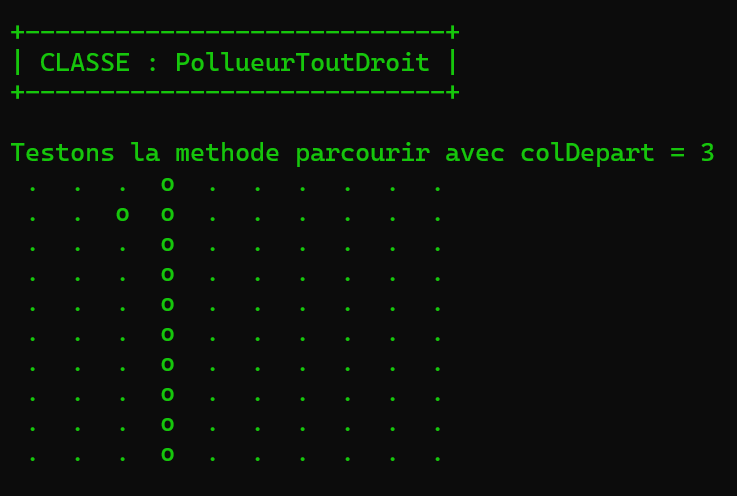
\includegraphics[scale=0.5]{../images/exo3.png}\\
On voit bien que toute les cases de la colonnes sont polluées.\\

\textcolor{red}{\textbf{\Large{Exercice 5 :}}}\\
Il s'agissait ici de créer la classe \textbf{PollueurSauteur} avec les différentes méthodes citées ci-dessus.\\
\begin{lstlisting}
// Test de la classe PollueurSauteur
System.out.println("+--------------------------+");
System.out.println("| CLASSE : PollueurSauteur |");
System.out.println("+--------------------------+\n");

// Creation et test d'un PollueurSauteur
PollueurSauteur polSauteur = new PollueurSauteur(0, 1, monde);
System.out.println("Testons la methode parcourir avec colDepart = 0 et deltax = 1");
polSauteur.parcourir();
System.out.println(monde.toString());
System.out.println("\n\n\n");
\end{lstlisting}

Dans ce code nous avons créé un objet \textbf{polSauteur}.\\
Par la suite, nous appelons la méthode \textbf{parcourir} sur l'objet créé pour que le robot se deplace dans le monde en sautant d'une colonne a l'autre et pollue les cases rencontrées\\
Enfin, on affiche le monde grâce à la méthode \textbf{toString}\\

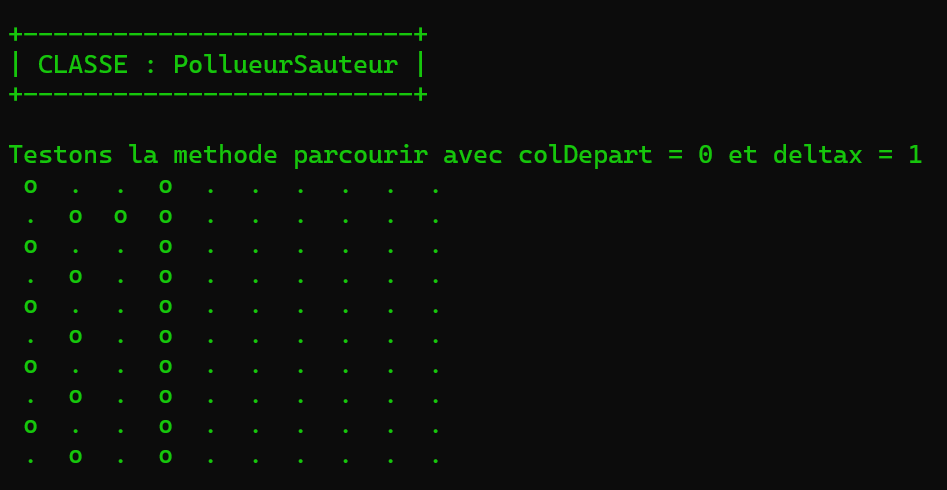
\includegraphics[scale=0.5]{../images/exo5.png}\\
On voit bien que le robot se deplace dans le monde en sautant d'une colonne a l'autre et pollue les cases rencontrées\\

\textcolor{red}{\textbf{\Large{Exercice 6 :}}}\\
Il s'agissait ici de créer la classe \textbf{RobotNettoyeur} avec les différentes méthodes citées ci-dessus.\\
\begin{lstlisting}
// Test de la classe RobotNettoyeur
System.out.println("+-------------------------+");
System.out.println("| CLASSE : RobotNettoyeur |");
System.out.println("+-------------------------+\n");

// Creation et test d'un RobotNettoyeur
System.out.println("Testons la methode parcourir :");
System.out.println("Affichons d'abord la matrice ");
System.out.println(monde.toString());
RobotNettoyeur robNettoyeur = new RobotNettoyeur(monde);
System.out.println("La matrice apres nettoyage ");
robNettoyeur.parcourir();
System.out.println(monde.toString());
System.out.println("\n\n\n");
\end{lstlisting}

Dans ce code nous avons créé un objet \textbf{robNettoyeur}.\\
Par la suite, nous redéfinissons la méthode \textbf{parcourir} sur l'objet créé pour qu'il se déplace dans le monde et nettoie les cases sales.\\
Enfin, on affiche le monde grâce à la méthode \textbf{toString}\\

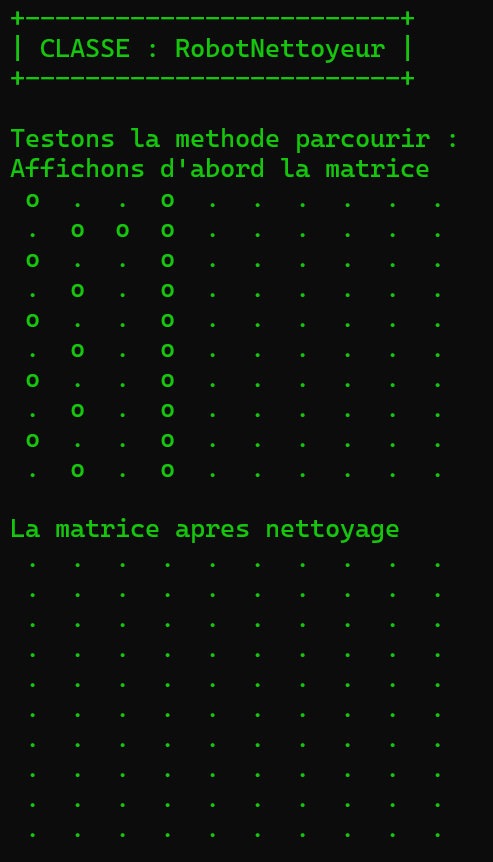
\includegraphics[scale=0.7]{../images/exo6.png}\\
On voit bien comment est le monde avant et après l'appel de la méthode \textbf{parcourir}.\\

\textcolor{red}{\textbf{\Large{Exercice 6 :}}}\\
Il s'agissait ici de créer la classe \textbf{NettoyeurDistrait} avec les différentes méthodes citées ci-dessus.\\
\begin{lstlisting}
	 //Test de la classe NettoyeurDistrait
	System.out.println("+----------------------------+");
	System.out.println("| CLASSE : NettoyeurDistrait |");
	System.out.println("+----------------------------+\n");
	
	//Creation et test d'un NettoyeurDistrait
	System.out.println("Testons la methode parcourir : ");
	System.out.println("Affichons d'abord la matrice ");
	p.parcourir();
	System.out.println(monde.toString());
	NettoyeurDistrait netDistrait = new NettoyeurDistrait(monde);
	System.out.println("La matrice apres nettoyage ");
	netDistrait.parcourir();
	System.out.println(monde.toString());
	System.out.println("\n\n\n");
\end{lstlisting}

Dans ce code nous avons créé un objet \textbf{netDistrait}.\\
Par la suite, nous redéfinissons la méthode \textbf{parcourir} sur l'objet créé.\\ Cette méthode alterne entre nettoyer une case sale et ne rien faire pour chaque case rencontrée.
Enfin, on affiche le monde grâce à la méthode \textbf{toString}\\

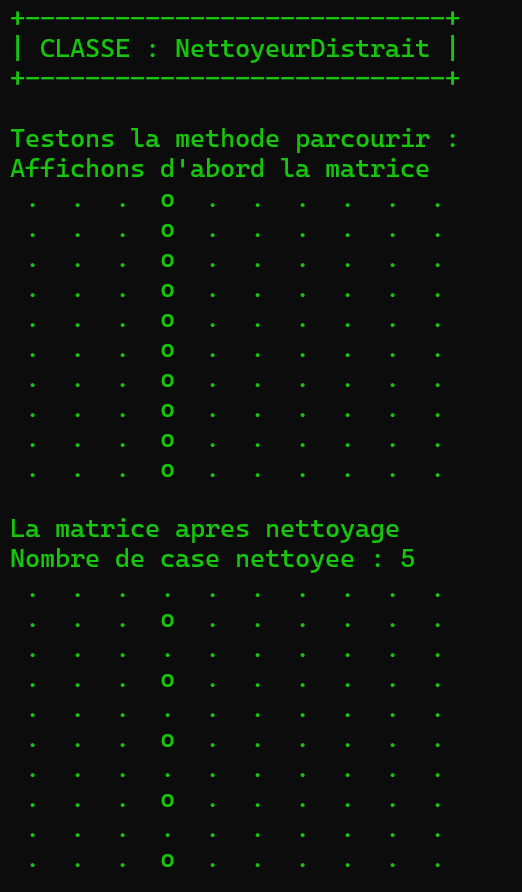
\includegraphics[scale=0.7]{../images/exo7.png}\\
On voit bien que le nettoyeur n'enlève qu’un papier	sur	deux.

\textcolor{red}{\section*{Archives :}}
\textbf{\large{Commandes : }}\\
\textcolor{red}{\textbf{jar cvf RobotsPollueursArchives Mondepackage Robotpackage PollueurToutDroitpackage Robotpollueurpackage PollueurSauteurpackage RobotNettoyeurpackage NettoyeurDistraitpackage}}

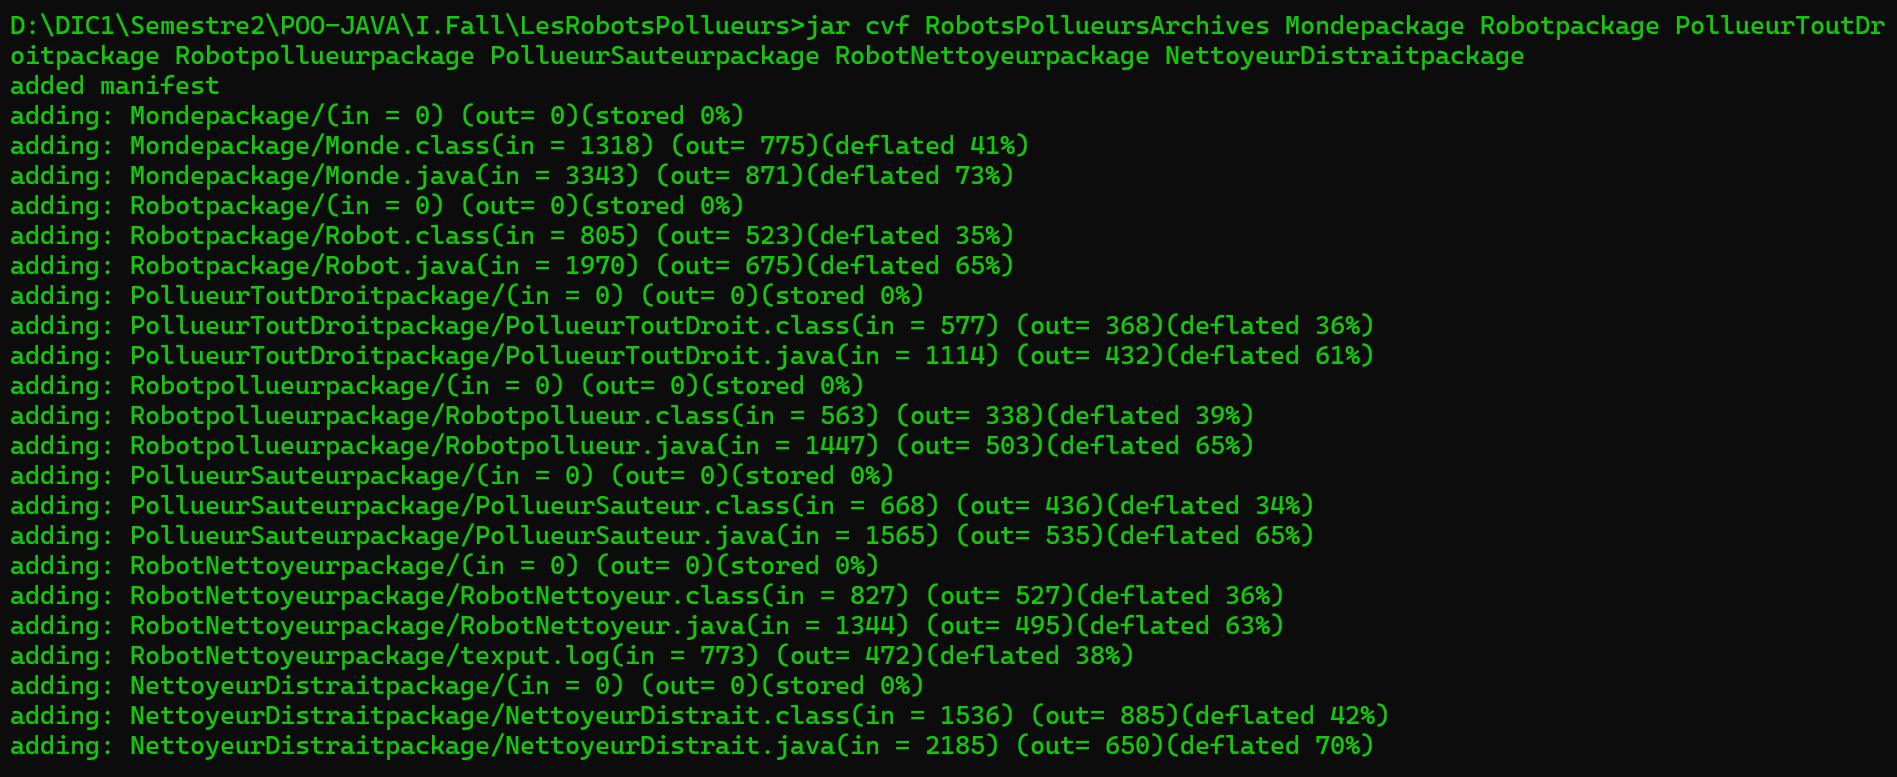
\includegraphics[scale=0.4]{../images/archive.png}\\

\textcolor{red}{\section*{Documentation	API	de	chaque	projet	(package) :}}
\textbf{\large{Commandes : }}\\
\textcolor{red}{\textbf{javadoc -d docs -sourcepath D:$\backslash$DIC1$\backslash$Semestre2$\backslash$POO-JAVA$\backslash$I.Fall$\backslash$LesRobotsPollueurs Mondepackage Robotpackage PollueurToutDroitpackage Robotpollueurpackage PollueurSauteurpackage RobotNettoyeurpackage NettoyeurDistraitpackage}}

\textcolor{red}{\section*{Dépot GitHub :}}
\url{https://github.com/MarieWalyFall/LesRobotsPollueurs}
\end{document}
							
